\documentclass[tikz]{standalone}

\usepackage{tikz}
\usetikzlibrary{arrows.meta,calc,positioning}

\definecolor{DarkNavy}{HTML}{0C122B}
\definecolor{CrispWhite}{HTML}{FFFFFF}
\definecolor{Aqua}{HTML}{009ee3}
\definecolor{SkyBlue}{HTML}{59bdf7}
\definecolor{Caribbean}{HTML}{35cdb4}
\definecolor{Sunshine}{HTML}{ffbc29}
\definecolor{IndianRed}{HTML}{ec6469}
\definecolor{Cornflower}{HTML}{4a4ad8}
\definecolor{SoftGray}{HTML}{706f6f}

\newcommand{\mlpnode}[3][DarkNavy]{%
  \tikz[baseline=(base.base),x=1.1mm,y=1.0mm,line width=0.25pt,>=Latex]{
    \node[inner sep=0,outer sep=0] (base) at (0,0) {};
    \node[font=\scriptsize,text=#1,anchor=east] at (-6,0) {#2};
    \node[font=\scriptsize,text=#1,anchor=west] at (5,0) {#3};
    \draw[-Latex,#1] (-6.2,0) -- (-4.2,0);
    \draw[-Latex,#1] (4.2,0) -- (6.2,0);
    \foreach \y in {-1,1} {
      \filldraw[fill=Cornflower,draw=DarkNavy] (-2.7,\y) circle (0.5);
    }
    \foreach \y in {-2,0,2} {
      \filldraw[fill=Sunshine,draw=DarkNavy] (0,\y) circle (0.5);
    }
    \filldraw[fill=Caribbean,draw=DarkNavy] (2.7,0) circle (0.5);
    \foreach \yin in {-1,1} {
      \foreach \yhid in {-2,0,2} {
        \draw[#1] (-2.7,\yin) -- (0,\yhid);
      }
    }
    \foreach \yhid in {-2,0,2} {
      \draw[#1] (0,\yhid) -- (2.7,0);
    }
  }%
}

\begin{document}
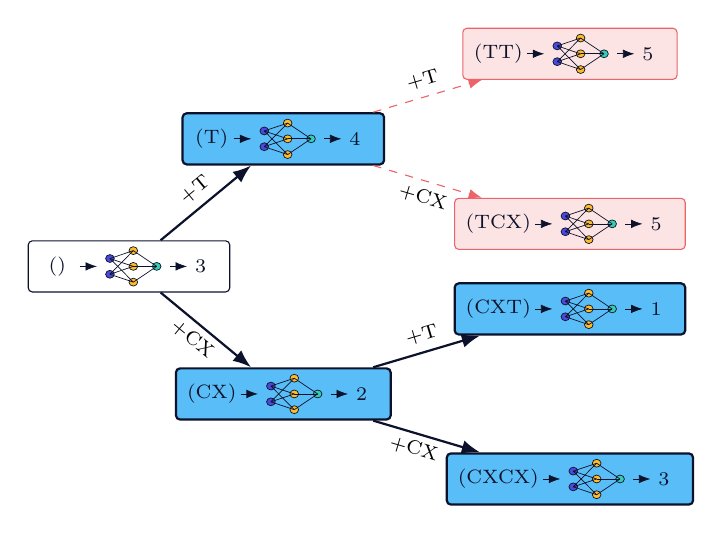
\begin{tikzpicture}[
  x=2.8cm,
  y=1.8cm,
  >=Latex,
  node/.style={rectangle,rounded corners=1.5pt,draw=DarkNavy,minimum width=6mm,minimum height=5mm,inner sep=2pt,font=\small},
  best/.style={node,fill=SkyBlue,thick},
  pruned/.style={node,draw=IndianRed,text=DarkNavy,fill=IndianRed,fill opacity=0.18,text opacity=1,draw opacity=1},
  edge/.style={-Latex,draw=DarkNavy,thick},
  pruned edge/.style={-Latex,draw=IndianRed,dashed},
  label/.style={font=\footnotesize},
  edge label/.style={font=\scriptsize,fill=CrispWhite,inner sep=1pt,sloped}
]
  \node[node] (s) at (0,0) {\mlpnode{()}{3}};

  \node[best] (a) at (0.7,0.9) {\mlpnode{(T)}{4}};
  \node[best] (b) at (0.7,-0.9) {\mlpnode{(CX)}{2}};
  \node[pruned] (d) at (2,1.5) {\mlpnode[DarkNavy]{(TT)}{5}};
  \node[pruned] (e) at (2,0.3) {\mlpnode[DarkNavy]{(TCX)}{5}};
  \node[best] (f) at (2,-0.3) {\mlpnode{(CXT)}{1}};
  \node[best] (g) at (2,-1.5) {\mlpnode{(CXCX)}{3}};
  \draw[edge] (s) -- node[edge label,midway,above=2pt] {+T} (a);
  \draw[edge] (s) -- node[edge label,pos=0.46,below=1.4pt] {+CX} (b);
  \draw[pruned edge] (a) -- node[edge label,midway,above=2pt] {+T} (d);
  \draw[pruned edge] (a) -- node[edge label,midway,below=2pt] {+CX} (e);
  \draw[edge] (b) -- node[edge label,midway,above=2pt] {+T} (f);
  \draw[edge] (b) -- node[edge label,pos=0.42,below=1.4pt] {+CX} (g);
\end{tikzpicture}
\end{document}
